\documentclass{beamer}
\usepackage[T1]{fontenc} \usepackage{lmodern} \usepackage[utf8]{inputenc}
\usepackage[english]{babel} \usepackage{booktabs}
\usepackage{graphicx,subcaption} \usepackage{amssymb,amsmath}
\graphicspath{{figures/}}
\usepackage[citestyle=authoryear,bibstyle=authoryear,backend=biber,url=false,doi=false,isbn=false]{biblatex} \bibliography{refs}
\usepackage{hyperref}

% Make Adobe Reader use the RGB rendering model for pages with transparency.
\pdfpageattr{/Group << /S /Transparency /I true /CS /DeviceRGB>>}

\mode<presentation>{
	\usetheme{Malmoe}
	\usecolortheme{beaver}
	\setbeamertemplate{footline}[page number]
	\setbeamertemplate{navigation symbols}{}
}

%------------------------------------------------

\DeclareMathOperator*{\diag}{diag}
\DeclareMathOperator*{\argmin}{arg\,min}
\DeclareMathOperator*{\spn}{span}
\newcommand{\G}{\mathcal{G}}
\newcommand{\V}{\mathcal{V}}
\newcommand{\E}{\mathcal{E}}
\newcommand{\bO}{\mathcal{O}}
\newcommand{\R}{\mathbb{R}}

\newcommand{\good}[1]{{\color[rgb]{0.2,0.6,0.2}#1}}
\newcommand{\bad}[1]{{\color{red}#1}}
\newcommand{\txt}[1]{\hspace{.5cm} \text{#1} \hspace{.5cm}}
\newcommand{\define}[1]{\item{\usebeamercolor[fg]{enumerate item}#1}:}
\newcommand{\HRule}{{\usebeamercolor[bg]{subsection in head/foot} \rule{\linewidth}{0.5mm}}}

%------------------------------------------------

\begin{document}

\begin{frame}[plain]
	%\titlepage
	\begin{center}

		\textsc{\large A Network Tour of Data Science}\\
		\vspace{0.7cm}

		\HRule
		\vspace{0.65cm}
		{
			\usebeamercolor[fg]{frametitle}
			%\textsc{\Large Practical Informations}\\
			\textsc{\Large Lab Sessions}\\
			%\textsc{\Large Laboratories}\\
			\vspace{0.4cm}
		}
		\HRule
		\vspace{1.0cm}

		\hspace{0.5cm}
		\begin{minipage}{0.4\linewidth}
			\footnotesize
			\textbf{Teachers} \\
			Pierre \textsc{Vandergheynst} \\
			Pascal \textsc{Frossard} \\
		\end{minipage}
		\begin{minipage}{0.4\linewidth}
			\footnotesize
			\textbf{Assistants} \\
			Michaël \textsc{Defferrard} \\
			Effrosyni \textsc{Simou} \\
			Hermina \textsc{Petric Maretić} \\
		\end{minipage}

		\vspace{0.7cm}
		\footnotesize EPFL LTS2 \& LTS4 laboratories\\
		\vspace{0.3cm}
		\footnotesize September 22, 2017

	\end{center}
\end{frame}

%------------------------------------------------

\begin{frame}
	\frametitle{Data Scientist}
	\begin{figure}
		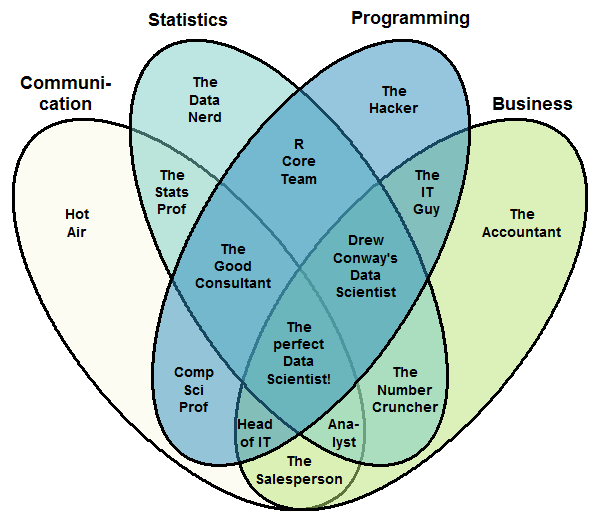
\includegraphics[height=0.8\textheight]{data_scientist}
	\end{figure}
\end{frame}

%------------------------------------------------

\begin{frame}
	\frametitle{Goal}
	\begin{center}
		Apply the material learned in class in a Data Science context.
	\end{center}
	\vfill
	During the labs, we will:
	\begin{itemize}
		\item Demo tools, e.g.\ how to manipulate a graph in Python.
		\item Demo techniques, e.g.\ how to collect data from Twitter.
		\item Explain the assignments and give directions.
		\item Answer questions about the assignments and project.
	\end{itemize}
	\vfill
	We expect you to:
	\begin{itemize}
		\item Bring your laptop.
		\item Work outside the hours on the assignments and project.
	\end{itemize}
\end{frame}

%------------------------------------------------

\begin{frame}
	\frametitle{Schedule (tentative)}
	\begin{description}
		\item[Sep 29] Data Science in Python
		\item[Oct  2] Lab 1 -- Network properties
		\item[Oct 13] Lab 1 -- Network properties
		\item[Oct 23] Lab 2 -- Network models
		\item[Oct 30] Lab 2 -- Network models
		\item[Nov  6] Lab 3 -- Spectral graph theory
		\item[Nov 13] Lab 3 -- Spectral graph theory
		\item[Nov 24] Project discussion
		\item[Nov 27] Lab 4 -- Graph signal processing
		\item[Dec  4] Lab 4 -- Graph signal processing
		\item[Dec 11] Lab 5 -- Machine learning
		\item[Dec 18] Lab 5 -- Machine learning
		\item[Dec 22] Project discussion
	\end{description}
\end{frame}

%------------------------------------------------

\begin{frame}
	\frametitle{Data Science Process}
	\begin{figure}
		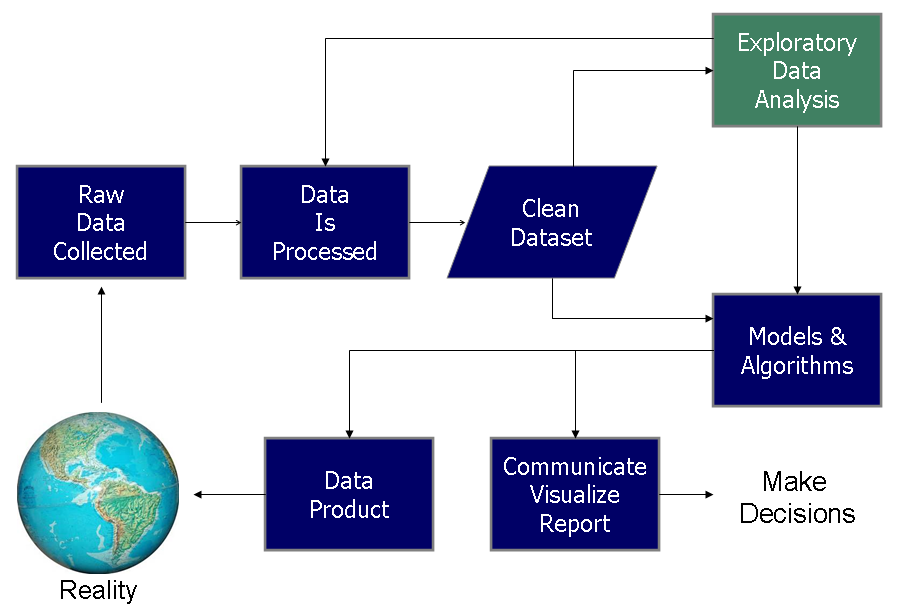
\includegraphics[width=\textwidth]{data_science_process}
	\end{figure}
\end{frame}

%------------------------------------------------

\begin{frame}
	\frametitle{Tools}
	\begin{center}
		Python scientific stack + \href{https://git-scm.com}{git}
	\end{center}
	\vfill
	To be installed with \href{https://www.anaconda.com/download}{Anaconda}:
	\begin{itemize}
		\item \href{https://www.python.org}{Python}: programming language
		\item \href{https://ipython.org}{IPython}: interactive computing
		\item \href{http://www.numpy.org}{NumPy}: N-dimensional arrays
		\item \href{https://www.scipy.org/scipylib/index.html}{SciPy}: scientific computing
		\item \href{https://matplotlib.org}{matplotlib}: visualization
		\item \href{https://pandas.pydata.org}{pandas}: data analysis
		\item \href{https://networkx.github.io}{NetworkX}: network science
		\item \href{https://graph-tool.skewed.de}{graph-tool}: network science
		\item \href{https://github.com/epfl-lts2/pygsp}{PyGSP}: graph signal processing
	\end{itemize}
\end{frame}

%------------------------------------------------

\begin{frame}
	\frametitle{Grading}
	\begin{enumerate}
		\item 50\% assignments (reports) \\
		$\rightarrow$ the continuous evaluation.
		\vspace{2em}
		\item 50\% project (report \& presentation) \\
		$\rightarrow$ the final exam!
	\end{enumerate}
\end{frame}

%------------------------------------------------

\begin{frame}
	\frametitle{Assignments}
	\begin{enumerate}
		\item Template notebook with instructions given on Githbub.
		\item Two weeks to complete.
		\item At least one lab session to ask questions.
		\item Completed notebook to be handled on Moodle.
		\item Solutions posted on Github.
		\item Grades given on Moodle.
	\end{enumerate}
	\vfill
	Topics from lectures, with a Data Science taint:
	\begin{enumerate}
		\item Network properties
		\item Network models
		\item Spectral Graph Theory
		\item Graph Signal Processing
		\item (Machine Learning)
	\end{enumerate}
\end{frame}

%------------------------------------------------

\begin{frame}
	\frametitle{Project}
	\begin{enumerate}
		\define{Proposal} define a problem you are interested in.
			\begin{itemize}
				\item Single page document. Organize yourselves in groups.
				\item Deadline in November (to be confirmed). Upload on Moodle.
				\item Not graded. Discussion with TAs will follow.
			\end{itemize}
		\vfill
		\define{Report} your solution, using the theory seen in class and the
			practical skills trained during labs.
			\begin{itemize}
				\item Jupyter notebook with text, math, code, analyzes and
					results.
				\item Deadline in January (to be confirmed). Upload on Moodle.
				\item Graded.
			\end{itemize}
		\vfill
		\define{Presentation} impress us!
			\begin{itemize}
				\item Presentation of 15 minutes in front of the class.
				\item Held in January (to be confirmed).
				\item Graded.
			\end{itemize}
	\end{enumerate}
\end{frame}

%------------------------------------------------

\begin{frame}
	\begin{figure}
		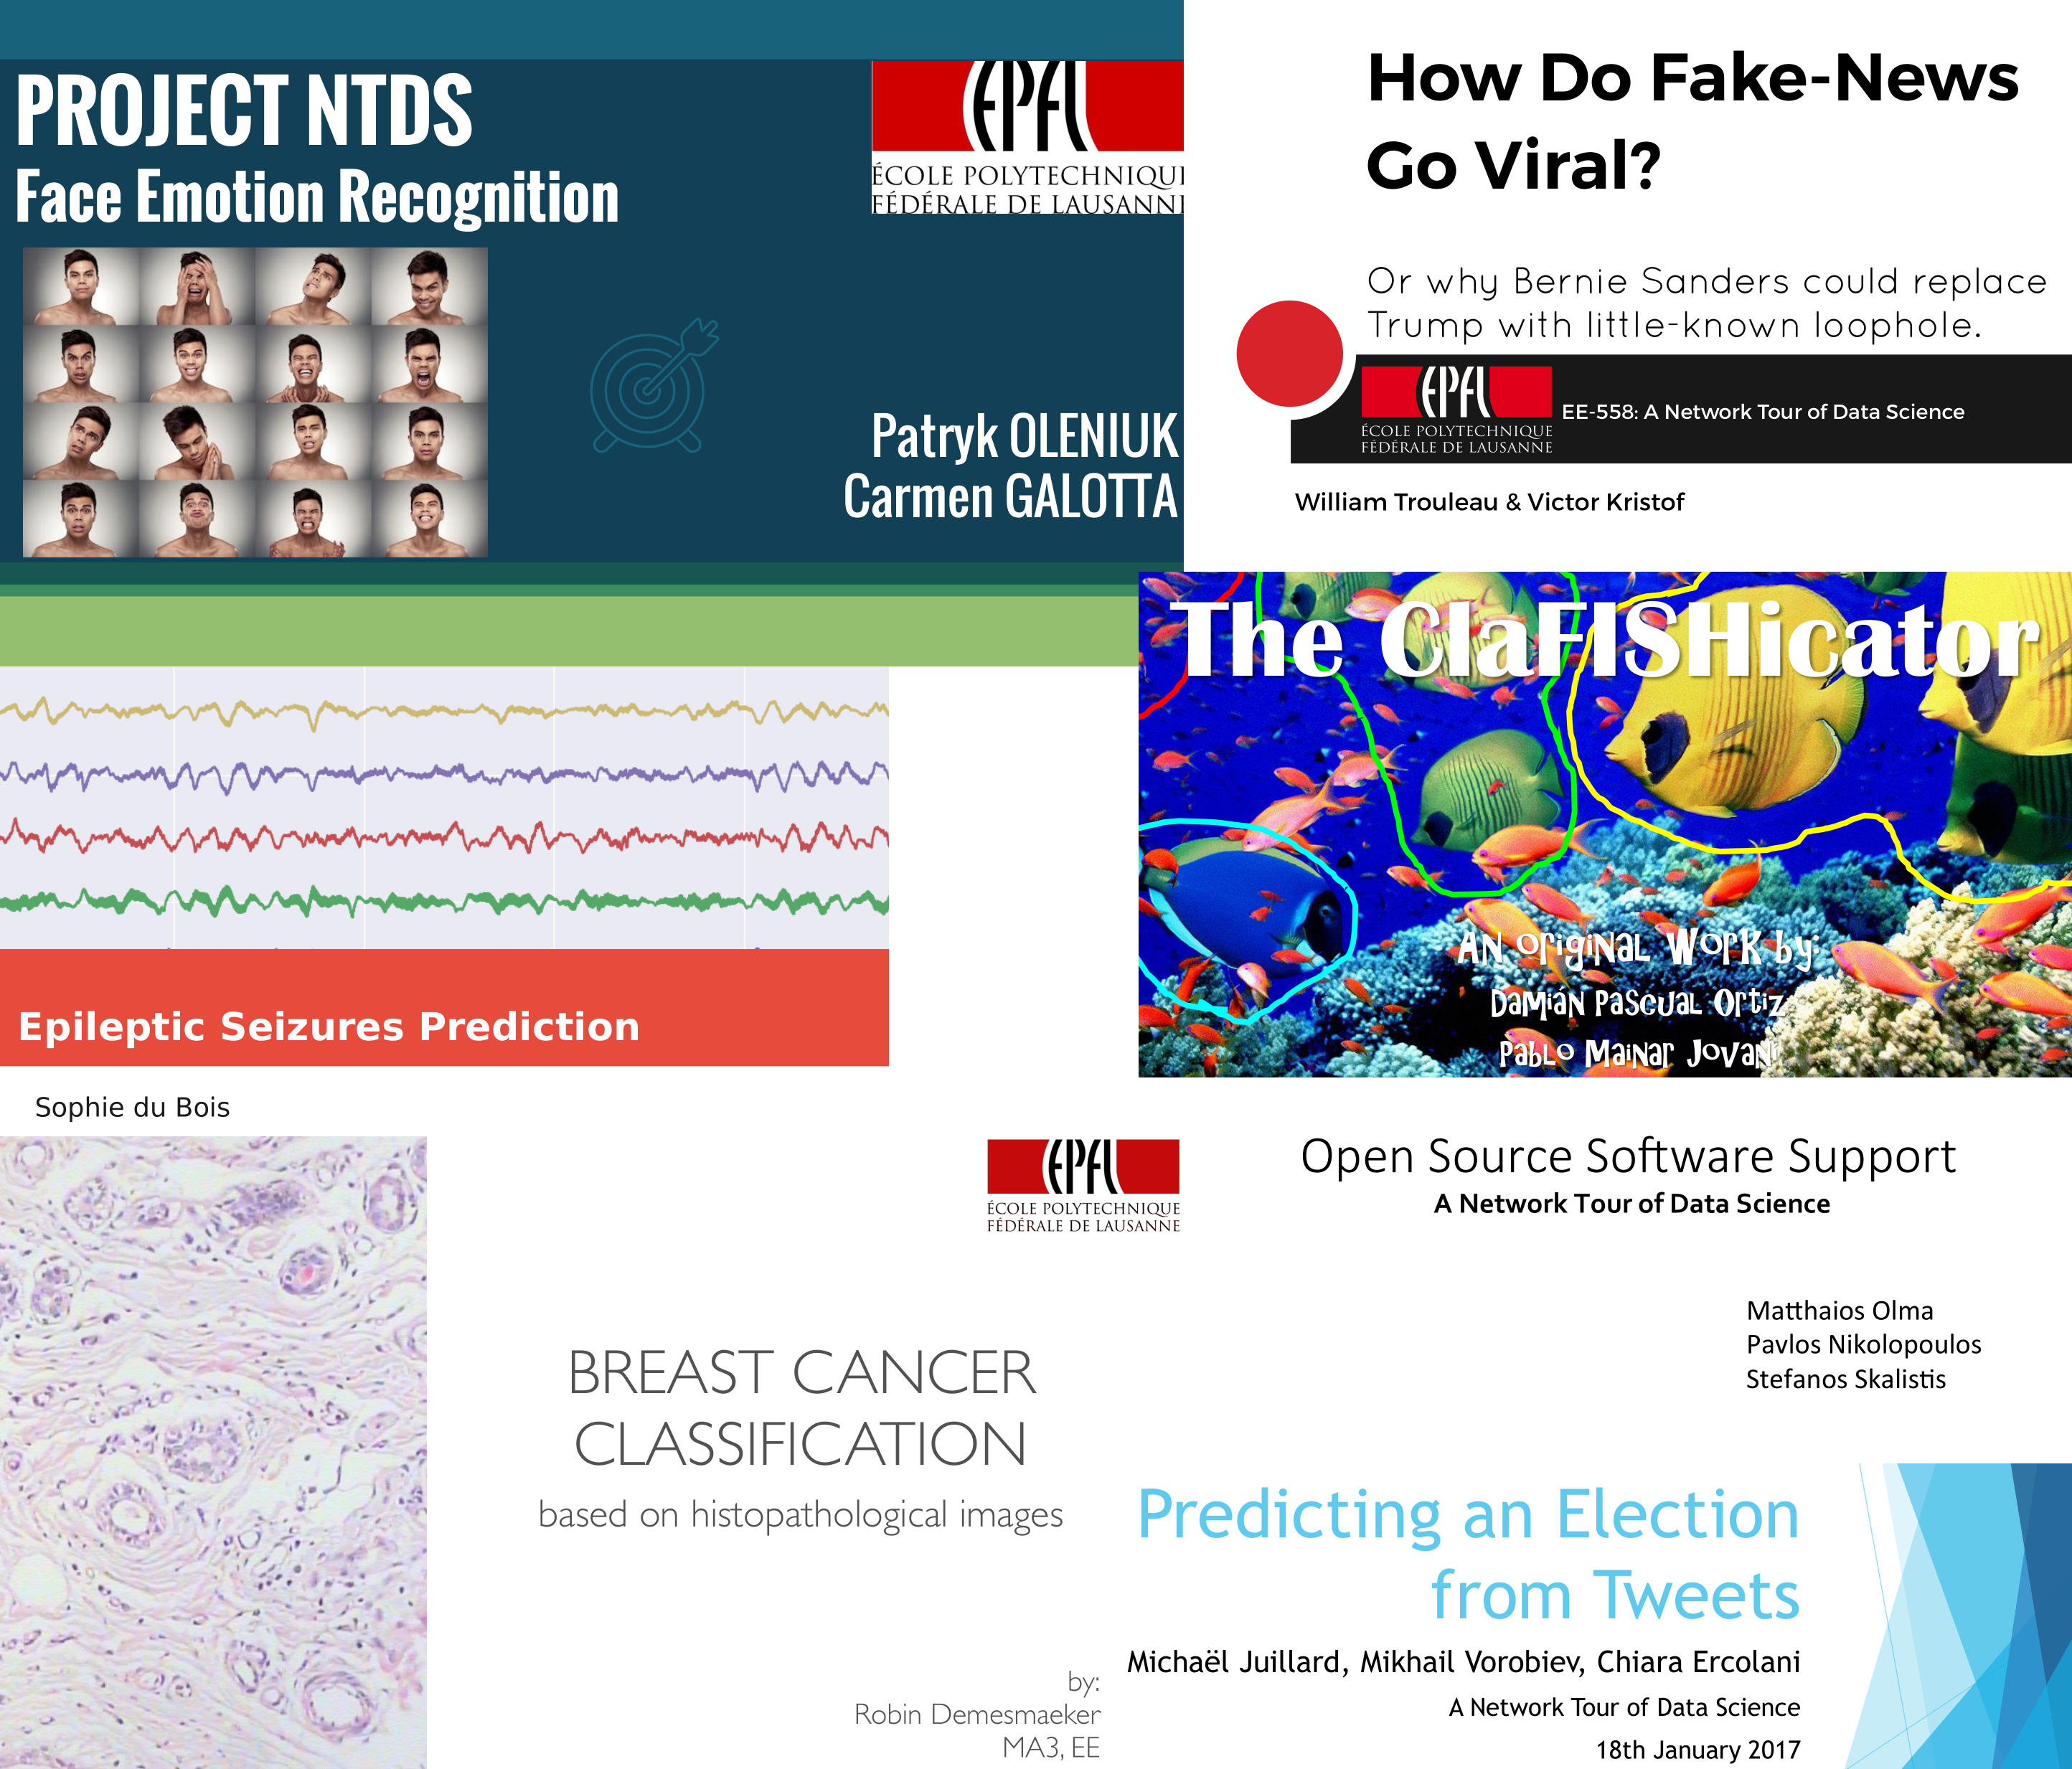
\includegraphics[width=0.9\textwidth]{projects_2016}
	\end{figure}
\end{frame}

%------------------------------------------------

\begin{frame}
	\begin{figure}
		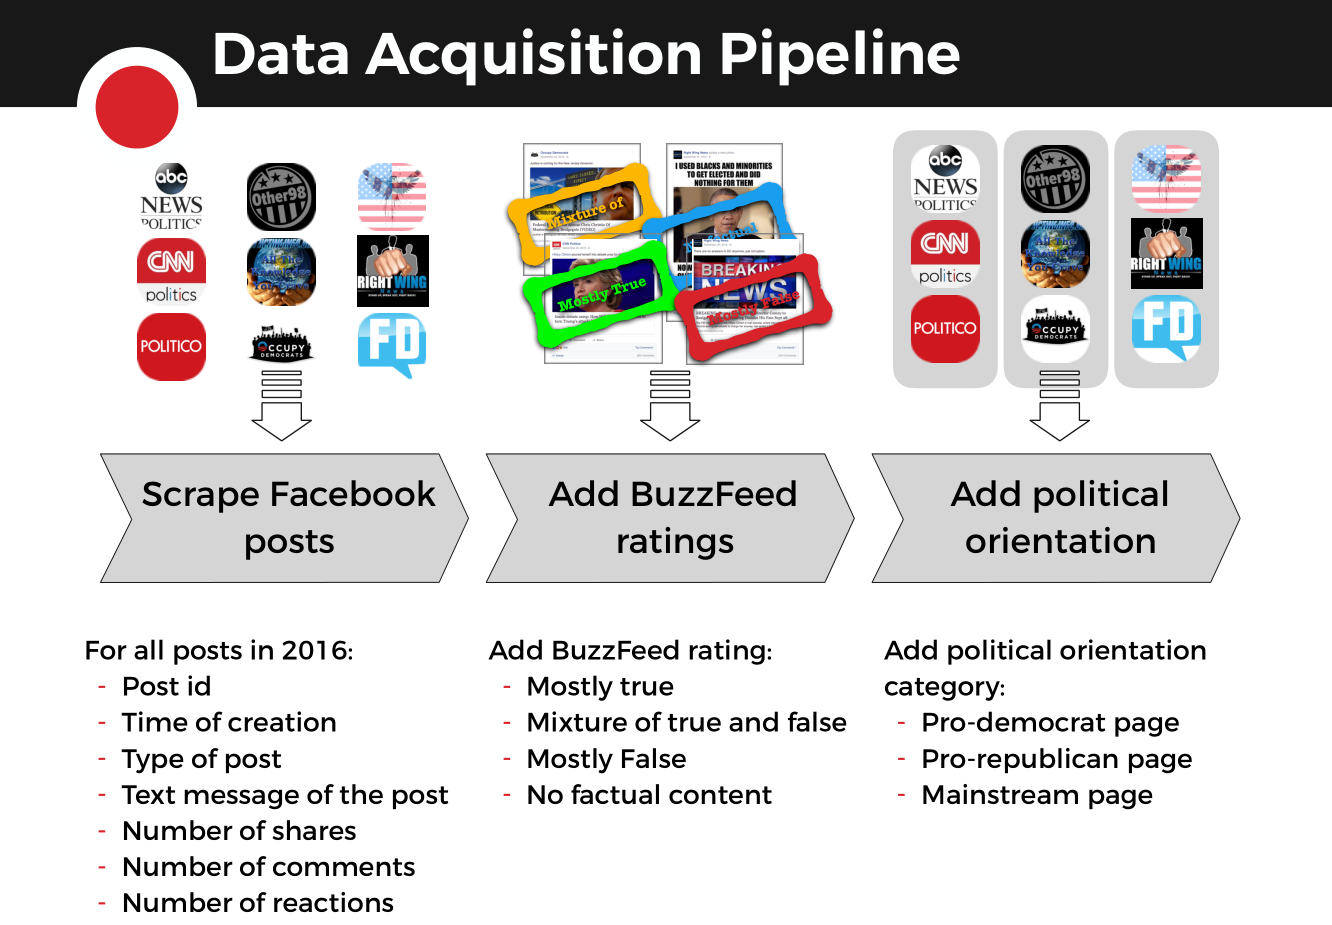
\includegraphics[width=\textwidth]{fake_news_1}
	\end{figure}
\end{frame}

%------------------------------------------------

\begin{frame}
	\begin{figure}
		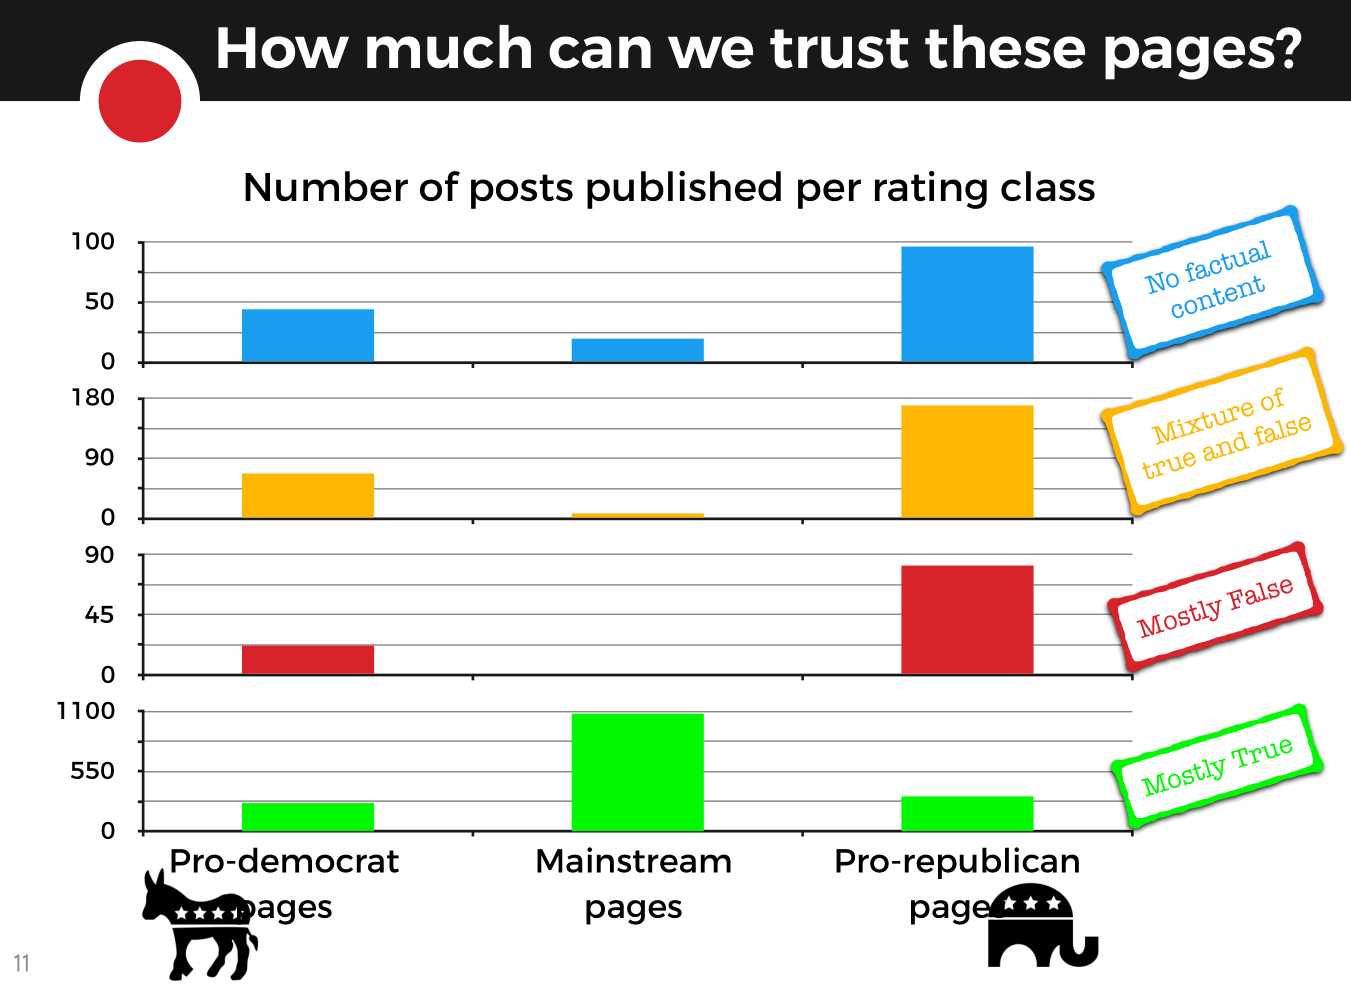
\includegraphics[width=\textwidth]{fake_news_2}
	\end{figure}
\end{frame}

%------------------------------------------------

\begin{frame}
	\begin{figure}
		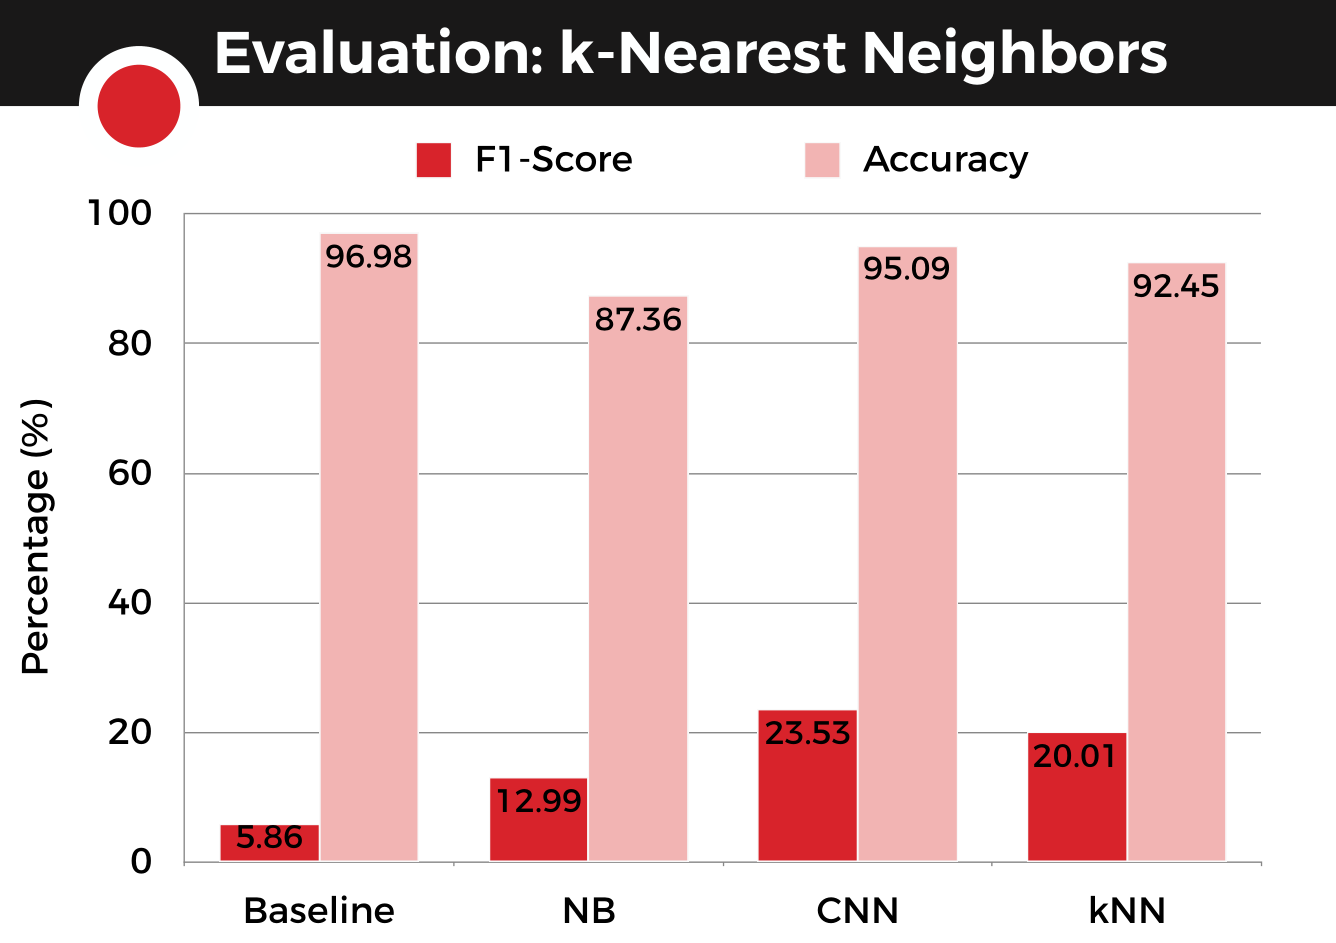
\includegraphics[width=\textwidth]{fake_news_3}
	\end{figure}
\end{frame}

%------------------------------------------------

\begin{frame}
	\frametitle{Online}
	Moodle: {\small \url{https://moodle.epfl.ch/course/view.php?id=15299}}
	\begin{itemize}
		\item Slides.
		\item Grades.
		\item Official announcements.
		\item Discussion forum.
	\end{itemize}
	\vspace{1em}
	GitHub: {\small \url{https://github.com/mdeff/ntds_2017}}
	\begin{itemize}
		\item Installation instructions.
		\item Demos.
		\item Assignments.
		\item Projects.
	\end{itemize}
	\vfill
	\begin{center}
		\Huge Questions?
	\end{center}
\end{frame}

%------------------------------------------------

\end{document}
